% diagram_flux_lora_stack.png
% FLUX.2-klein flow model as a vertical stack of layer groups with two side inputs.
% Canvas: 15.23 cm x 5.00 cm (= \textwidth of the deck, height <= 5.0 cm).
\documentclass[border=0pt,11pt]{standalone}
\usepackage[T1]{fontenc}
\usepackage{lmodern}
\renewcommand{\familydefault}{\sfdefault}
\usepackage{tikz}
\usetikzlibrary{positioning,arrows.meta}

\definecolor{primaryNavy}{RGB}{24,24,27}
\definecolor{secondaryNavy}{RGB}{63,63,70}
\definecolor{mutedGray}{RGB}{248,250,252}
\definecolor{ruleGray}{RGB}{226,232,240}

\tikzset{
  box/.style={draw=secondaryNavy, line width=0.6pt, fill=mutedGray, rectangle,
              inner xsep=5pt, inner ysep=2.5pt, align=center,
              text=primaryNavy, font=\small},
  ar/.style={draw=secondaryNavy, line width=0.6pt,
             -{Latex[length=1.4mm,width=1.0mm]}},
  dline/.style={draw=secondaryNavy, line width=0.6pt, dashed},
  din/.style={draw=secondaryNavy, line width=0.6pt, dashed,
              -{Latex[length=1.4mm,width=1.0mm]}},
  alab/.style={text=primaryNavy, font=\small, fill=white, inner sep=1.5pt},
}

\begin{document}
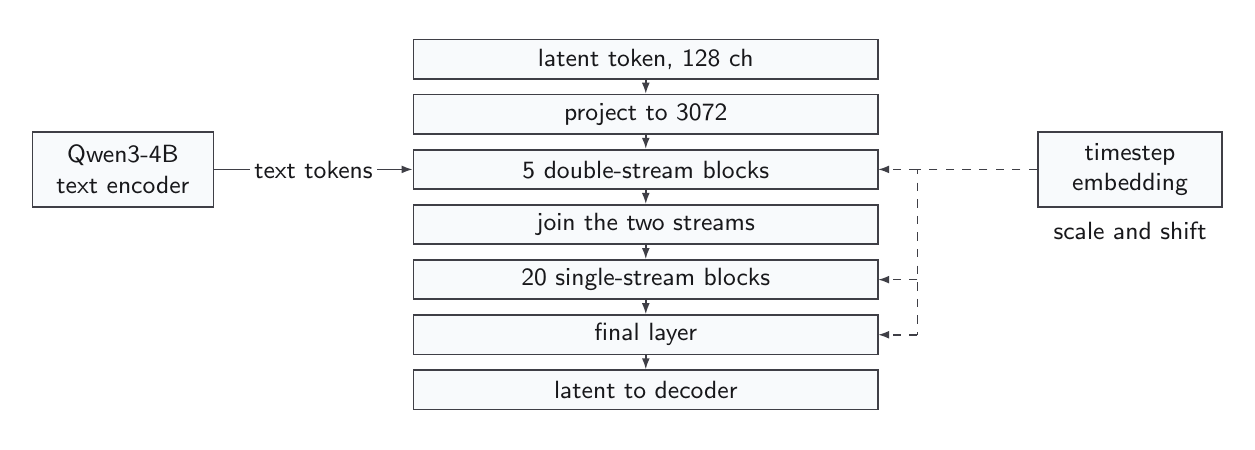
\begin{tikzpicture}[x=1cm,y=1cm]
\useasboundingbox (0,0) rectangle (15.23,5.00);
\fill[white] (0,0) rectangle (15.23,5.00);

% ---------------- flow model stack (top to bottom) ----------------
\node[box, minimum width=5.90cm, minimum height=0.50cm] (s1) at (7.85,4.60) {latent token, 128 ch};
\node[box, minimum width=5.90cm, minimum height=0.50cm] (s2) at (7.85,3.90) {project to 3072};
\node[box, minimum width=5.90cm, minimum height=0.50cm] (s3) at (7.85,3.20) {5 double-stream blocks};
\node[box, minimum width=5.90cm, minimum height=0.50cm] (s4) at (7.85,2.50) {join the two streams};
\node[box, minimum width=5.90cm, minimum height=0.50cm] (s5) at (7.85,1.80) {20 single-stream blocks};
\node[box, minimum width=5.90cm, minimum height=0.50cm] (s6) at (7.85,1.10) {final layer};
\node[box, minimum width=5.90cm, minimum height=0.50cm] (s7) at (7.85,0.40) {latent to decoder};

\draw[ar] (s1.south) -- (s2.north);
\draw[ar] (s2.south) -- (s3.north);
\draw[ar] (s3.south) -- (s4.north);
\draw[ar] (s4.south) -- (s5.north);
\draw[ar] (s5.south) -- (s6.north);
\draw[ar] (s6.south) -- (s7.north);

% ---------------- text encoder input (left) ----------------
\node[box, minimum width=2.30cm, minimum height=0.95cm] (enc) at (1.21,3.20) {Qwen3-4B\\text encoder};
\draw[ar] (enc.east) -- (s3.west);
\node[alab] at (3.63,3.20) {text tokens};

% ---------------- timestep input (right) ----------------
\node[box, minimum width=2.34cm, minimum height=0.95cm] (ts) at (14.00,3.20) {timestep\\embedding};

% single branched dashed path into the stack
\draw[dline] (ts.west) -- (11.30,3.20) -- (11.30,1.10);
\draw[din] (11.30,3.20) -- (10.80,3.20);
\draw[din] (11.30,1.80) -- (10.80,1.80);
\draw[din] (11.30,1.10) -- (10.80,1.10);

\node[alab] at (14.00,2.42) {scale and shift};

\end{tikzpicture}
\end{document}
